\subsection{A LIfe Question}
\begin{frame}[t]{A Life Question}
\begin{columns}[T, onlytextwidth]
\column{0.5\textwidth}
The \Sun\ and \Moon\ are both VOC, with the \Moon\ being first to leave her sign so looked to her first with the \Sun\ as sharer even though he is stronger, being angular.\\
\vspace{0.25cm}
\Moon\ 28 \Aries\ $\Rightarrow$ \Taurus \\
$\Rightarrow$ \Square\ \Mercury\ 2 \Aquarius\ \\
\hspace{1em} (\Moon\ commits her disposition, no reception) \\
\Mercury\ is joined to, and received by, \Saturn\ (4 \Aries) \\
\hspace{1em}(\Mercury\ is within 2° of a perfect \Sextile, already engaged) \\
therefore \Saturn\ signifies the person's health and good fortune\\
\vspace{0.25cm}
\Sun\ 24 \Aquarius\ $\Rightarrow$ \Pisces \\
$\Rightarrow$ \Sextile\ \Jupiter\ 9 \Taurus\  (with reception) \\
so the \Sun\ also signifies health and good fortune \\
\vspace{0.25cm}
Both L1 and the \Moon\ indicate the same for the person's health and fortune.
\column{0.5\textwidth}
\begin{center}
{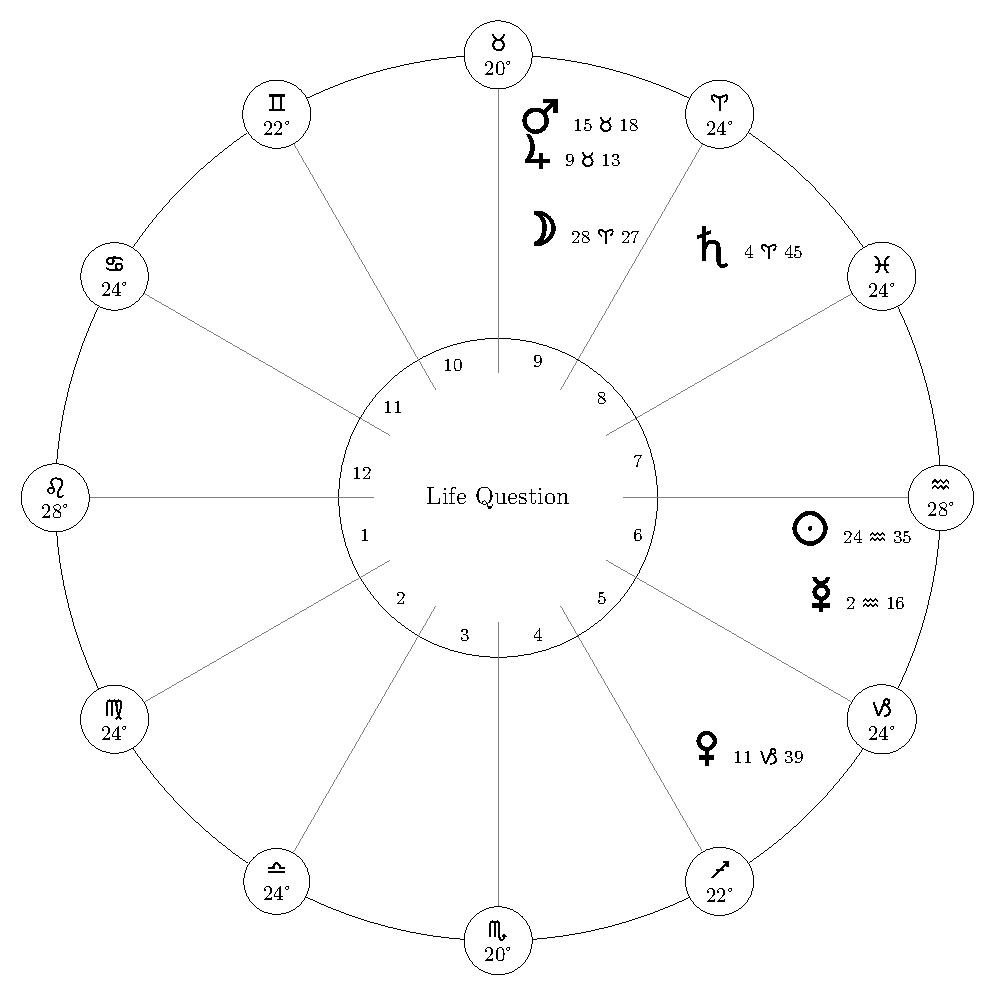
\includegraphics[width=0.9\textwidth]{charts/22-chart-life}}
\end{center}
\end{columns}
\end{frame}
% -------------------------------------------------------
\begin{frame}[t]{A Life Question Continued}

Wanting to know when the sickness would lessen, Masha'Allah says he next looked at the House of Sickness, the 6th, which was ruled by \Saturn, and \Venus\ (11 \Capricorn) was separated from \Saturn\ by 7° and moving to \Trine\ \Mars\ (15 \Taurus) with each receiving the other; \Mars\ receiving \Venus\ in his exaltation, \Venus\ receiving \Mars\ in her domicile.

This \textsl{"signified a lessening of pain and the arrival of health"}

\end{frame}